%%%%%%%%%%%%%%%%%%%%%%%%%%%%%%%%%%%%%%%%%%%%%%%%%%%%%%%%%%%%%%%%%%%%%%%%%%%%%%%%
%%%%%%%%%%%%%%%%%%%%%%%%%%%%%%%%%%%%%%%%%%%%%%%%%%%%%%%%%%%%%%%%%%%%%%%%%%%%%%%%
\documentclass[11pt]{article}

\usepackage[numbers,square]{natbib}
\renewcommand\cite[1]{(\citet{#1})}
\usepackage
[
        a4paper,% other options: a3paper, a5paper, etc
        left=2cm,
        right=2.5cm,
        top=3cm,
        bottom=4cm,
        % use vmargin=2cm to make vertical margins equal to 2cm.
        % us  hmargin=3cm to make horizontal margins equal to 3cm.
        % use margin=3cm to make all margins  equal to 3cm.
]
{geometry}
\usepackage{color}
\usepackage{chemarr}
\usepackage{amssymb}
\usepackage{graphicx}
\usepackage{textcomp} 
\usepackage[gen]{eurosym}
\usepackage{amsmath}
\usepackage[margin=1.5cm]{caption}
\usepackage{amsmath,mathtools}
\usepackage{subcaption}
%\setlength{\belowcaptionskip}{-5pt}
%\setlength{\abovecaptionskip}{-8pt}
\usepackage{enumitem}

%\usepackage[autolinebreaks,useliterate]{mcode}
\usepackage[usenames, dvipsnames]{xcolor}
\colorlet{shadecolor}{gray!5}
\usepackage{listings}
\lstset{ 
  language=R,                     % the language of the code
  basicstyle=\scriptsize\ttfamily, 	  % the size of the fonts
  numbers=left,                   % where to put the line-numbers
  numberstyle=\tiny\color{Blue},  % the style that is used for the line-numbers
  stepnumber=1,                   % the step between two line-numbers.
  numbersep=5pt,                  % how far the line-numbers are from the code
  backgroundcolor=\color{shadecolor},  % choose the background color.
  showspaces=false,               % show spaces adding particular underscores
  showstringspaces=false,         % underline spaces within strings
  showtabs=false,                 % show tabs within strings adding particular underscores
  frame=tb,                   	  % adds a frame around the code
  rulecolor=\color{Black},        % if not set, the frame-color may be changed on line-breaks within not-black text (e.g. commens (green here))
  tabsize=2,                      % sets default tabsize to 2 spaces
  captionpos=b,                   % sets the caption-position to bottom
  breaklines=true,                % sets automatic line breaking
  breakatwhitespace=false,        % sets if automatic breaks should only happen at whitespace
  keywordstyle=\color{RoyalBlue}, % keyword style
  commentstyle=\color{OliveGreen},% comment style
  stringstyle=\color{ForestGreen} % string literal style
}



%%%%%%%%%%%%%%%%%%%%%%%%%%%%%%%%%%%%%%%%%%%%%%%%%%%%%%%%%%%%%%%%%%%%%%%%%%%%%%%%
\title{\textbf{Comparing BC mixing state from CAMChem to SP2 measurements}}
\author{Yinrui Li}
\date{}


%\maketitle


\begin{document}
\maketitle
%%%%%%%%%%%%%%%%%%%%%%%%%%%%%%%%%%%%%%%%%%%%%%%%%%%%%%%%%%%%%%%%%%%%%%%%%%%%%%%%



\section{SP2 Measurement} 

The SP2 instrument measures BC particles in the diameter range from approximately 90 to 400~nm, which is unlikely to represent the total ambient number and mass concentrations of BC (Reddington et al., 2013). 
In order to compare CAMChem model simulated BC with observations, we estimated the mass fraction of modeled BC in the size range (90--400~nm) corresponding to SP2 measurement.


 
\section{Estimating the mean BC core diameter in primary carbon mode and in accumulation mode} 

A 4-mode version of the modal aerosol model (MAM4) is applied in CAMChem1.2.2. BC is emitted to the primary carbon mode, and then is transferred to the accumulation mode by condensation of $\rm{H_2SO_4}$, $\rm{NH_3}$ and $\rm{SOA}$ and by coagulation (Liu et al., 2012). In primary carbon mode, particles consist of externally mixed BC and OC, whereas in accumulation mode, particles consist of internally mixed BC and non-BC material.
\bigskip
\noindent SP2 measures the mass size distribution of the BC particle cores over a calibrated volume equivalent diameter (VED) range of 55--400~nm, and the number-detection efficiency at sea level pressure is reported to be one for BC above 90~nm VED (Schwarz et al., 2010a). So following Reddington et al., 2013, we use 90~nm as the lower bound here. 
\bigskip
\noindent Both modes assume lognormal distribution as is shown in table 1. $\sigma_{g}$ is fixed but geometric mean diameter can change according to total mass and total number of aerosol particles in that mode.

\begin{table}
	\begin{center}
		\begin{tabular}{c|c|c}
			\hline  
			MAM4 & $\sigma_{g}$ &  10th and 90th percentiles ($\mu m$)		\\   \hline
			Accumulation  & 1.8  &   0.058-0.27 		\\ \hline
			Primary Carbon   & 1.6  &  0.039-0.13  		\\
			\hline			
		\end{tabular}
	\end{center}
\caption{\label{tab:ozone} Parameters of Lognormal Distribution.}
\end{table}


\bigskip
\noindent The mean BC core diameter in accumulation mode is estimated as:
\begin{align*}
D_{\text{core}} = (D_{\text{mixed}}^3 \times f_{\text{BC}})^\frac{1}{3}, 
\end{align*}
where $D_{\text{core}}$ is the mean diameter of BC core,$D_{\text{mixed}}$ is the mean diameter of internally mixed particles (\textbf{extracted from model}), and $f_{\text{BC}}$ is the volume fraction of BC in accumulation mode.



 
\section{Compute Volume Fraction Corresponding to Lognormal Distribution}
The CDF of number distribution in the size range between $d_{1}$ and $d_{2}$ is:
\begin{align*}
N(d_{1}, d_{2}) = \frac{1}{\text{ln}\sigma_{\text{g}}\sqrt{2\pi}}\int_{d_{1}}^{d_{2}}e^-\frac{(\text{ln}r - \text{ln}r_{g})^2}{2\text{ln}^2\sigma_{\text{g}}}\text{d}(\text{ln}r),
\end{align*}
where $r_{g}$ is mean geometric diameter (extracted from model, varying temporally and spatially). 

\noindent The mean volume is proportional to function of the form:
\begin{align*}
V(d_{1}, d_{2}) &= \frac{1}{\text{ln}\sigma_{\text{g}}\sqrt{2\pi}}\int_{d_{1}}^{d_{2}}r^3e^-\frac{(\text{ln}r - \text{ln}r_{g})^2}{2\text{ln}^2\sigma_{\text{g}}}\text{d}(\text{ln}r)  \\
&=\frac{e^{\frac{k^2}{2}\text{ln}^2\sigma_{g}+k\text{ln}r_{g}}}{\text{ln}\sigma_{\text{g}}\sqrt{2\pi}}\int_{d_{1}}^{d_{2}}r^3e^-\frac{(\text{ln}r - \text{ln}r_{\text{gv}})^2}{2\text{ln}^2\sigma_{\text{g}}}\text{d}(\text{ln}r),
\end{align*}
where the volume mean diameter is of the form $\text{lnr}_{\text{gv}} = \text{lnr}_{\text{g}} + 3\text{ln}\sigma_{\text{g}}$.

\noindent So BC mass fraction (in the size range between 90--400~nm) in a mode is derived by:

\begin{align*}
F(\text{d}_{1}, \text{d}_{2}) &= \frac{\frac{1}{\text{ln}\sigma_{\text{g}}\sqrt{2\pi}}\int_{d_{1}}^{d_{2}}r^3e^-\frac{(\text{ln}r - \text{ln}r_{g})^2}{2\text{ln}^2\sigma_{\text{g}}}\text{d}(\text{ln}r)}
{\frac{1}{\text{ln}\sigma_{\text{g}}\sqrt{2\pi}}\int_{0}^{+\infty}r^3e^-\frac{(\text{ln}r - \text{ln}r_{g})^2}{2\text{ln}^2\sigma_{\text{g}}}\text{d}(\text{ln}r)}  \\
&=\frac{\frac{e^{\frac{k^2}{2}ln^2\sigma_{g}+k\text{ln}r_{g}}}{\text{ln}\sigma_{\text{g}}\sqrt{2\pi}}\int_{d_{1}}^{d_{2}}e^-\frac{(\text{ln}r - \text{ln}r_{\text{gv}})^2}{2\text{ln}^2\sigma_{\text{g}}}\text{d}(\text{ln}r)}{\frac{e^{\frac{k^2}{2}ln^2\sigma_{g}+k\text{ln}r_{g}}}{\text{ln}\sigma_{\text{g}}\sqrt{2\pi}}\int_{0}^{+\infty}e^-\frac{(\text{ln}r - \text{ln}r_{\text{gv}})^2}{2\text{ln}^2\sigma_{\text{g}}}\text{d}(\text{ln}r)}\\
&=\frac{1}{\text{ln}\sigma_{\text{g}}\sqrt{2\pi}}\int_{d_{1}}^{d_{2}}e^-\frac{(\text{ln}r - \text{ln}r_{\text{gv}})^2}{2\text{ln}^2\sigma_{\text{g}}}\text{d}(\text{ln}r) \\
&=\frac{1}{2}[\text{erf}(\frac{\text{ln}d_{2} - \text{ln}r_{\text{gv}}}{\sqrt{2}\text{ln}\sigma})-\text{erf}(\frac{\text{ln}d_{1} - \text{ln}r_{\text{gv}}}{\sqrt{2}\text{ln}\sigma})],
\end{align*}




\bigskip
\bigskip
\bigskip
\begin{figure}[!h] 
	\begin{center}
		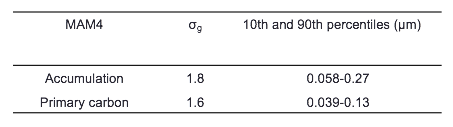
\includegraphics[width = 0.6\textwidth]{Rplot01}
		\caption[]{\label{fig_P1}BC mass in primary carbon mode (top) and in accumulation mode (bottom), for surface layer, March.}
	\end{center}
\end{figure}

\begin{figure}[!h] 
	\begin{center}
		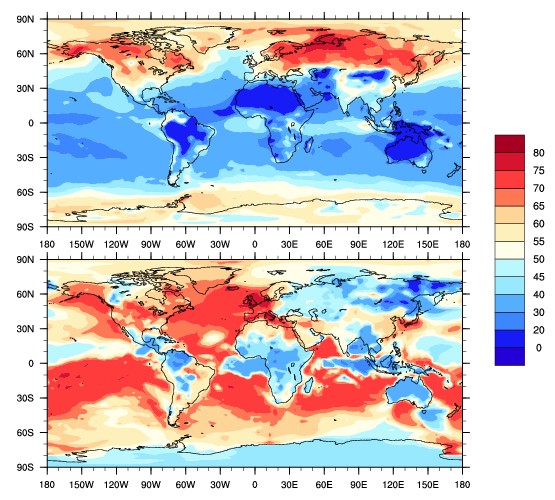
\includegraphics[width = 0.6\textwidth]{Rplot02}
		\caption[]{\label{fig_P2} BC mass fraction ($\%$) (between 90 and 400~nm) in primary carbon mode (top) and in accumulation mode (bottom), for surface layer, March.}
	\end{center}
\end{figure}


\noindent \textbf{Within the size range (90--400~nm)}, the ratio of BC mass in each mode to total BC mass is computed as:
\begin{align*}
f_{\text{accu}} = \frac{F_{\text{accu}}(d_{1}, d_{2})M_{\text{accu}}}{F_{\text{accu}}(\text{d}_{1}, d_{2})M_{\text{accu}}+F_{\text{pc}}(d_{1}, d_{2})M_{\text{pc}}}\\
f_{\text{pc}} = \frac{F_{\text{pc}}(d_{1}, d_{2})M_{\text{pc}}}{F_{\text{accu}}(d_{1}, d_{2})M_{\text{accu}}+F_{\text{pc}}(d_{1}, d_{2})M_{\text{pc}}}
\end{align*}
\[f_{\text{accu}} + f_{\text{pc}} = 1,\]

\noindent where $f_{\text{accu}}$ is the fraction of BC mass in accumulation mode, $f_{\text{pc}}$ is the fraction of BC mass in primary carbon mode, $M_{\text{accu}}$ and $M_{\text{pc}}$ are BC mass in accumulation mode and primary carbon mode respectively.

\noindent BC mass fraction ($F_{\text{pc}}(90~nm, 400~nm)$ and $F_{\text{accu}}(90~nm, 400~nm)$) are shown in Figure~\ref{fig_P2}, for primary carbon mode (upper panel) and for accumulation mode (lower panel). At the surface, SP2 would see most of BC in primary carbon mode at high latitudes ($\textgreater$60$\%$). At low and middle latitudes, this portion is lower than 40$\%$ for most regions. SP2 can capture most of BC in accumulation mode when it is distant from source regions (e.g., throughout the oceans). We also observe that little BC could be seen in either mode for Central Africa. Fractions in two panels should not add up to 1.

\noindent $f_{\text{pc}}$ and $f_{\text{accu}}$ are shown in the upper and lower panels in Figure~\ref{fig_P3} respectively. They indicate the mixing state of BC particles that can be captured by SP2 measurements. Most of them ($\textgreater$60$\%$) are internally mixed in low and middle latitudes, and are externally mixed in high latitudes. The fraction can vary spatially for Arctic region (between 40$\%$ and 70$\%$), which should be taken into consideration when comparing modeled BC with SP2 measurements. Fractions in two panels should add up to 1. 


\begin{figure}[!h] 
	\begin{center}
		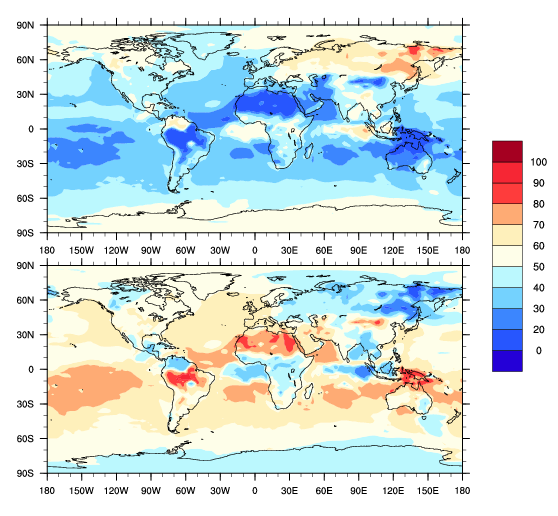
\includegraphics[width = 0.6\textwidth]{Rplot03}
		\caption[]{\label{fig_P3} Ratio of BC mass ($\%$) within SP2 size range to total BC mass within SP2 size range, in primary carbon mode (top) and accumulation mode (bottom), for surface layer, March.}
	\end{center}
\end{figure}





\clearpage
\noindent \textbf{References. }

C. L. Reddington, G. McMeeking, G. W. Mann1, H. Coe, M. G. Frontoso, D. Liu, M. Flynn, D. V. Spracklen, and K. S. Carslaw: The mass and number size distributions of black carbon aerosol over Europe, Atmos. Chem. Phys., 13, 4917-4939, doi:10.5194/acp-13-4917-2013, 2013

Liu, X., Easter, R. C., Ghan, S. J., Zaveri, R., Rasch, P., Shi, X., Lamarque, J.-F., Gettel- man, A., Morrison, H., Vitt, F., Conley, A., Park, S., Neale, R., Hannay, C., Ekman, A. M. L., Hess, P., Mahowald, N., Collins, W., Iacono, M. J., Bretherton, C. S., Flanner, M. G., and Mitchell, D.: Toward a minimal representation of aerosols in climate models: description and evaluation in the Community Atmosphere Model CAM5, Geosci. Model Dev., 5, 709–739, doi:10.5194/gmd-5-709-2012, 2012.

Schwarz, J. P., Spackman, J. R., Gao, R. S., Perring, a. E., Cross, E., Onasch, T. B., Ahern, a., Wrobel, W., Davidovits, P., Olfert, J., Dubey, M. K., Mazzoleni, C., and Fahey, D. W.: The Detection Efficiency of the Single Particle Soot Photometer, Aerosol Sci. Technol., 44, 612–628, doi:10.1080/02786826. 2010.481298, 2010a.









%%%%%%%%%%%%%%%%%%%%%%%%%%%%%%%%%%%%%%%%%%%%%%%%%%%%%%%%%%%%%%%%%%%%%%%%%%%%%%%%



\end{document}
%%%%%%%%%%%%%%%%%%%%%%%%%%%%%%%%%%%%%%%%%%%%%%%%%%%%%%%%%%%%%%%%%%%%%%%%%%%%%%%%
%%%%%%%%%%%%%%%%%%%%%%%%%%%%%%%%%%%%%%%%%%%%%%%%%%%%%%%%%%%%%%%%%%%%%%%%%%%%%%%%